%%%%%%%%%%%%%%%%%%%%%%%%%%%%%%%%%%%%%%%%%
% Imperial Placement Report Template 
% LaTeX Template
% Version 1.0 (28/06/16)
% Version 1.1 (20/01/28) 
% Modified by Aufar Laksana into a lab report template
% For academic use only
%%%%%%%%%%%%%%%%%%%%%%%%%%%%%%%%%%%%%%%%%
%----------------------------------------------------------------------------------------
%	PACKAGES AND OTHER DOCUMENT CONFIGURATIONS
%----------------------------------------------------------------------------------------

\documentclass[12pt,a4paper]{report}
\usepackage[english]{babel}
\usepackage[utf8x]{inputenc}
\usepackage{amsmath}
\usepackage{amsfonts}
\usepackage{graphicx}
\usepackage{fancyhdr}
\usepackage[colorinlistoftodos]{todonotes}
\usepackage[toc,page]{appendix}
\usepackage{listings}
\usepackage[page]{totalcount}
\usepackage{color}
\usepackage{geometry}
\usepackage{caption}
\usepackage{subcaption}
\usepackage{float}
\usepackage[bottom]{footmisc}
\usepackage{diagbox}
\usepackage{gensymb}
\usepackage{mathpazo}

\usepackage{natbib} 



\definecolor{mygreen}{rgb}{0,0.6,0}
\definecolor{mygray}{rgb}{0.5,0.5,0.5}
\definecolor{mymauve}{rgb}{0.58,0,0.82}
\definecolor{mylilas}{RGB}{170,55,241}

\pagestyle{fancy}
\fancyhf{}
\lhead{Final Year Project}
\rhead{Interim Report}
\rfoot{\thepage\ / \totalpages}

% \geometry{headheight=15pt}
% \geometry{footskip=0.4in}
% \geometry{textheight=694pt}
% \geometry{textwidth=400pt}



\lstset{ %
  basicstyle=\small,
  backgroundcolor=\color{white},   % choose the background color; you must add \usepackage{color} or \usepackage{xcolor}; should come as last argument
  breaklines=true,                 % sets automatic line breaking
  captionpos=b,                    % sets the caption-position to bottom
  commentstyle=\color{mygreen}\ttfamily\small,    % comment style
  escapeinside={\%*}{*)},          % if you want to add LaTeX within your code
  extendedchars=true,              % lets you use non-ASCII characters; for 8-bits encodings only, does not work with UTF-8
  frame=shadowbox,	                   % adds a frame around the code
  rulesepcolor=\color{teal},
  keepspaces=true,                 % keeps spaces in text, useful for keeping indentation of code (possibly needs columns=flexible)
  keywordstyle=\color{blue},       % keyword style
  language=C,                 % the language of the code
  morekeywords={*,...},            % if you want to add more keywords to the set
  numbers=left,                    % where to put the line-numbers; possible values are (none, left, right)
  rulecolor=\color{black},         % if not set, the frame-color may be changed on line-breaks within not-black text (e.g. comments (green here))
  showspaces=false,                % show spaces everywhere adding particular underscores; it overrides 'showstringspaces'
  showstringspaces=false,          % underline spaces within strings only
  showtabs=false,                  % show tabs within strings adding particular underscores
  stringstyle=\color{mymauve},     % string literal style
  tabsize=2,	                   % sets default tabsize to 2 spaces
}
\lstdefinelanguage{Mymatlab}{
    language=Matlab,%
    %basicstyle=\color{red},
    basicstyle=\ttfamily\footnotesize,
    breaklines=true,%
    morekeywords={matlab2tikz},
    keywordstyle=\color{blue},%
    morekeywords=[2]{1}, keywordstyle=[2]{\color{black}},
    identifierstyle=\color{black},%
    stringstyle=\color{mylilas},
    commentstyle=\color{mygreen},%
    showstringspaces=false,%without this there will be a symbol in the places where there is a space
    numbers=left,%
    numberstyle={\tiny \color{black}},% size of the numbers
    numbersep=9pt, % this defines how far the numbers are from the text
    emph=[1]{for,end,break},emphstyle=[1]\color{red}, %some words to emphasise
    %emph=[2]{word1,word2}, emphstyle=[2]{style},    
}
\lstdefinelanguage{TI}{
  sensitive = true,
  keywords={MVC,MVK,MVKLH,LDDW,LDW,NOP,STW,ZERO,LDDW,MPYDP,ADDDP,SUB,B},
  otherkeywords={% Operators
    >, <, ==
  },
  keywords = [2]{_circ_FIR_DP,loop,lend},
  keywordstyle=\color{blue},
  keywordstyle=[2]\color{purple},% for example
  numbers=left,
  numberstyle=\scriptsize,
  stepnumber=1,
  numbersep=8pt,
  showstringspaces=false,
  breaklines=true,
  frame=shadowbox,	                   % adds a frame around the code
  rulesepcolor=\color{teal},
  comment=[l]{;},
  morecomment=[s]{/*}{*/},
  commentstyle=\color{mygreen}\ttfamily\small,
  stringstyle=\color{red}\ttfamily,
  morestring=[b]',
  morestring=[b]"
  }


\begin{document}

\begin{titlepage}


\newcommand{\HRule}{\rule{\linewidth}{0.5mm}} % Defines a new command for the horizontal lines, change thickness here
\setlength{\topmargin}{0in}
\center % Center everything on the page
 
\vspace*{-3cm}
 
\begin{minipage}{0.4\textwidth}
\begin{flushleft} \large
\hspace*{-0.5cm}
%\includegraphics[scale=0.14]{Imperial.png}\\
\end{flushleft}
\end{minipage}
~
\begin{minipage}{0.5\textwidth}
\begin{flushright} \large
\hspace*{2cm}
% \includegraphics[scale=0.4]{dsk6713.jpg}\\
\end{flushright}
\end{minipage}\\[1cm]
%----------------------------------------------------------------------------------------
%	HEADING SECTIONS
%----------------------------------------------------------------------------------------

\textsc{\LARGE Imperial College of Science, Technology and Medicine}\\[1.5cm] % Name of your university/college
\textsc{\Large Department of Electrical and Electronic Engineering}\\[0.8cm] % Major heading such as course name
\textsc{\Large  Final Year Project}\\[0.8cm] % Minor heading such as course title

%----------------------------------------------------------------------------------------
%	TITLE SECTION
%----------------------------------------------------------------------------------------

\addvspace{1.8em}

\HRule \\[0.2cm]
{ \huge \bfseries Interim Report:\\ Augmented Reality for Human Robotic Interaction }\\[0.2cm] % Title of your document
\HRule \\[1cm]
 
%----------------------------------------------------------------------------------------
%	AUTHOR SECTION
%----------------------------------------------------------------------------------------

\begin{flushleft}

\large \emph{Authors:} \\
Aufar \textsc{Laksana} \\
CID: 01093575\\

\addvspace{0.6em}

\large \emph{Project Supervisor:} \\
Dr. Yiannis Demiris\\

\addvspace{0.6em}

%\large \emph{Project Second Marker:} \\
%Dr. David Thomas\\

\addvspace{1.8em}

\end{flushleft}

% \begin{minipage}{1\textwidth}
% 	\begin{center}
% 		\frame{\includegraphics[scale=0.9]{declare.png}}\\
% 	\end{center}
% \end{minipage}\\[1cm]


\vspace*{3em}

%----------------------------------------------------------------------------------------
%	DATE SECTION
%----------------------------------------------------------------------------------------

{\large \today}\\[0.5cm] % Date, change the \today to a set date if you want to be precise


\vfill % Fill the rest of the page with whitespace
Shortcode: apl115 \\
\end{titlepage}

\addvspace{6em}

\renewcommand{\abstractname}{\LARGE Abstract}

\tableofcontents
\newpage

\setlength{\parindent}{0pt}
\setlength{\parskip}{10pt}

\chapter{Introduction and Requirements}

\section{Introduction}
This report was written as part of the Final Year Project for the MEng. Electronic \& Information Engineering course. The project is supervised by Dr. Yiannis Demiris at the Imperial College London. The content of the report covers the research and progress of the project so far, between October 2018 until January 2019.

\section{Motivation}
A study on powered wheelchair users showed that there were approximately 3.6 million wheelchair users in the United States alone \citep{Kairy2014}. The study also showed that approximately 30\% of the users were operating powered wheelchairs (PWCs) or scooters, and that similar data had been reported in Europe. According to a report examining the recent trends amongst adults aged 65 and older in the United States, the number of elderly adults is projected to more than double from 46 million to over 98 million by 2060; due to increased life expectancy stemming from better healthcare and a reduction in mortality rate at older ages \citep{Mather2015}. As a result of the growing elderly population, it is likely that the number of powered mobility devices will continue to grow.

The study by \cite{Kairy2014} also highlights the problems faced by powered wheelchair users (PWUs). PWUs are often afraid of navigating in crowded areas, or are unable to operate their device safely, due to visual, motor and cognitive disabilities. In order to address these issues, the implementation of smart or intelligent wheelchairs has been proposed. These smart wheelchairs will help the users by providing services such as navigation assistance, allowing the user to carry out daily activities with more ease. An example of navigation assistance is collaborative control, \cite{Carlson2012} which utilizes a smart system that recognizes and assists the user when they require help, by manipulating the control signals of the powered wheelchair.

Within the Personal Robotics Lab at the Imperial College London, a lot of work has been done on enhancing the powered wheelchair user experience. One approach, \cite{Zolotas2018} involves the use of an augmented reality (AR) headset to help the user understand their wheelchair's behaviour. The AR headset renders helpful indicators, such as the trajectory of the wheelchair and highlighting potential obstacle collisions.

This project explores the idea implementing a smart system that would further benefit PWUs, by allowing them to navigate in crowded areas and recognizing locations that are frequently visited, such as at home or the shopping mall, and building a map of the location to allow better navigation assistance. An AR headset can also be utilized to display the internal state of the smart wheelchair, such as highlighting objects that determine the frequently visited location, or alerting the user to people moving towards the wheelchair and rendering a suggested path to avoid collision.

\section{Project Specification}
The aim of this project is to design and build a system that will allow powered wheelchair users to more easily conduct routine tasks, such as navigating around the house, or other frequently visited locations, such as the grocery store.

This project involves several hardware components, all of which are available within the Personal Robotics Lab. The hardware includes the following, as well as the sensors already mounted on the wheelchair:

\begin{itemize}
	\item Powered Wheelchair
	\item Microsoft Hololens
	\item Cameras (Microsoft Kinect)
\end{itemize}


The system being developed is divided into two major parts, Robotic Behaviour and Augmented Reality Visualization.

\subsection{Robotic Behaviour}
The goal for this section of the project is to design and develop algorithms that will allow for assistive navigation on the powered wheelchair. The system will utilize sensors mounted on the wheelchair to build up a map of the surroundings. Objects in the surrounding area will be detected and marked as potential collisions, depending on the trajectory of the wheelchair. An extension is the ability to detect moving objects, such as people, calculating the trajectory of the object and deciding if a collision is imminent.

A major hardware component of this project is the Microsoft Hololens, a mixed reality headset that can be worn by the powered wheelchair user. The Hololens posses the ability to track the eye movements of the user. An interesting concept that can be explored is the ability to control the powered wheelchair using the eye-tracker, removing the need for a joystick. This would benefit users who lack the motor skills to operate a joystick. This feature can also be utilized to check if the user has noticed an object that may cause a collision. Should the user not see the object, the system will first highlight the object, before taking over from the user and altering the trajectory to avoid the object.

\subsection{Augmented Reality Visualization}
Using the Hololens, the goal of this section is to communicate to the user the internal state of the system controlling the powered wheelchair. Using augmented reality, visualizations will be rendered on the Hololens, allowing the user to understand the trajectory of the wheelchair, what potential collisions may occur. The system will also be able to take over control of the wheelchair, as such, it would be beneficial if a warning was displayed to the user right before the system takes over.

Other visualizations include highlighting moving objects and tracking them as they move across the field of vision of the user. Should the user not notice a moving object that may cause a collision, the Hololens will flash a warning and highlight the offending object in order to attract the attention of the user, allowing them to make adjustments themselves.

\newpage

\chapter{Literature Review}

\section{Object Detection}
In this project, the main purpose of object detection algorithms will be to identify objects of the class 'Human' in the surrounding area of the wheelchair. In order to tackle the problem of users being unwilling to navigate in crowded areas, a system must be implemented to help track and navigate around humans.

One of the modern approaches to detecting humans in an image from a camera is to use Deep Convolutional Neural Networks. Human detection,as stated by \cite{Vidanapathirana}, is a special case of Object Detection and Object Localization. The system would ideally be able to pinpoint the location of the human object relative to the wheelchair, in order to be able to calculate the trajectory of the person.

However, the use cases of object detection is not only limited to detecting humans. There has been research conducted into the use of object detection for recognizing the scene around a robot, ie. the system is able to identify the robot is now in a hallway \citep{Quattoni2009, Espinace2010}.

\subsection{Human Detection}
The main challenges with detecting humans in an image is the large variations in the appearance. A frontal view of a person may be recognized by the algorithm, but a side view may cause problems due to the algorithm not recognizing key features from a different angle \citep{Dalal2004}.

\paragraph{SIFT} A solution to this problem is outlined by \cite{Lowe2004}, in an approach named the Scale Invariant Feature Transform (SIFT), which transforms image data into co-ordinates which are scale invariant relative to local features. This method allows for a large number of features to be extracted from an image. The feature are also distinct, allowing for a single feature to be correctly matched with a low uncertainty against a database of existing features.

A large quantity of features is required for object detection, due to the often cluttered nature of the image. In order to detect a small object in the background, at least 3 features must be correctly matched for reliable identification. 

In order to perform object detection, SIFT features are first extracted from the training set of available images. A new image, in our case, a human torso/body, will be recognized by individually comparing the features in the test image with the features in the training set, in a Nearest Neighbours approach utilizing Euclidean distance. However, a drawback of using SIFT is the high computational cost of comparing the features \citep{Wang2011}.

\paragraph{YOLO}
You Only Look Once (YOLO) is a state of the art object detection system relying on a single neural network to predict bounding boxes around the objects \citep{Redmon2015}. The main advantage of YOLO is that it is extremely fast, as the name, the algorithm only looks once at an image to predict what objects are present.

\begin{figure}[h!]
	\begin{center}
		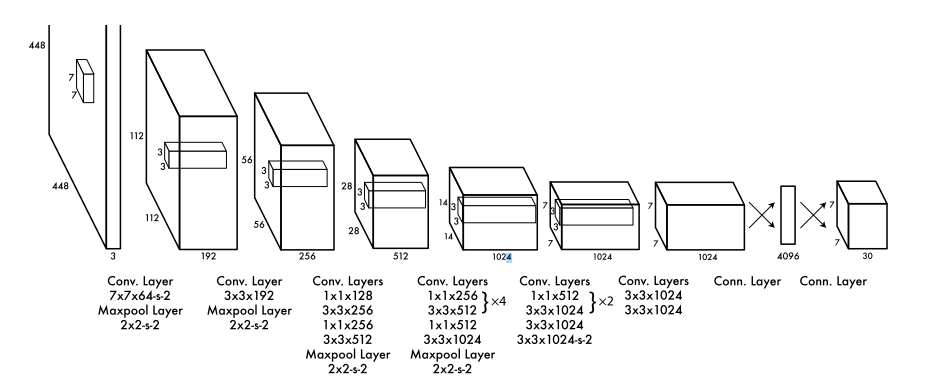
\includegraphics[scale=0.4]{Images/Literature/YOLO_Architecture.png}
		\caption{The YOLO architecture \citep{Redmon2015}}
	\end{center}
\end{figure}

The Convolutional Neural Network (CNN) in the YOLO system takes in an image and resizes it to 448x488 pixels. The image is then passed through the CNN layers and is output as a 7x7x30 tensor, containing the co-ordinates of the bounding boxes and the probability distributions over all the classes the network is trained on. 

The YOLO algorithm has been used to recognize human actions by \cite{Shinde2018}, using the LIRIS Human Activities dataset, which contain human actions such as shaking hands and entering rooms. It was found in the study that only a few frames of a streamed video is required for the YOLO algorithm to recognize the human actions.

\begin{figure}[h!]
	\begin{center}
		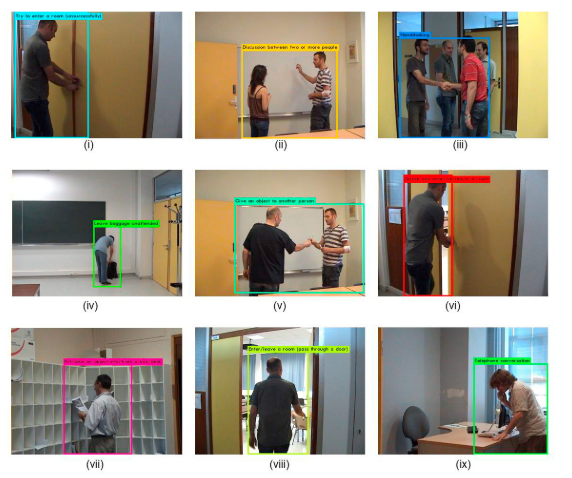
\includegraphics[scale=0.4]{Images/Literature/YOLO_Action_Recognition.png}
		\caption{The YOLO algorithm recognizing human actions \citep{Shinde2018}}
	\end{center}
\end{figure}

An extension of this work for the purposes of this project would be to detect humans walking towards the camera mounted on the wheelchair, in order to help with navigating through crowded areas.

\section{Camera Pose Estimation}

\section{Simultaneous Localization And Mapping (SLAM)}
The term mapping refers to a system that will create a map of the surrounding areas, by detecting objects such as walls and other obstacles. In order to help users navigate, the system must analyse the surroundings for potential dangers. As such, it is important to build up a thorough and complete map.

A fundamental method for robot navigation is the Simultaneous Localization And Mapping (SLAM) method. The process allows the system to predict the trajectory of the robot and the location of all objects on-line, without the need of an \textit{a priori} knowledge of the robots location \citep{Bailey2006a}. The method estimates the pose of the robot relative to landmarks which are detected. The popularity of SLAM increased with the emergence of indoor applications of robotic devices. For this project, it is expected that the user will be mostly navigating around the house or indoors, which rules out the use of GPS to bound the localization errors \citep{Cadena2016}.

%\begin{figure}[h!]
%	\begin{center}
%		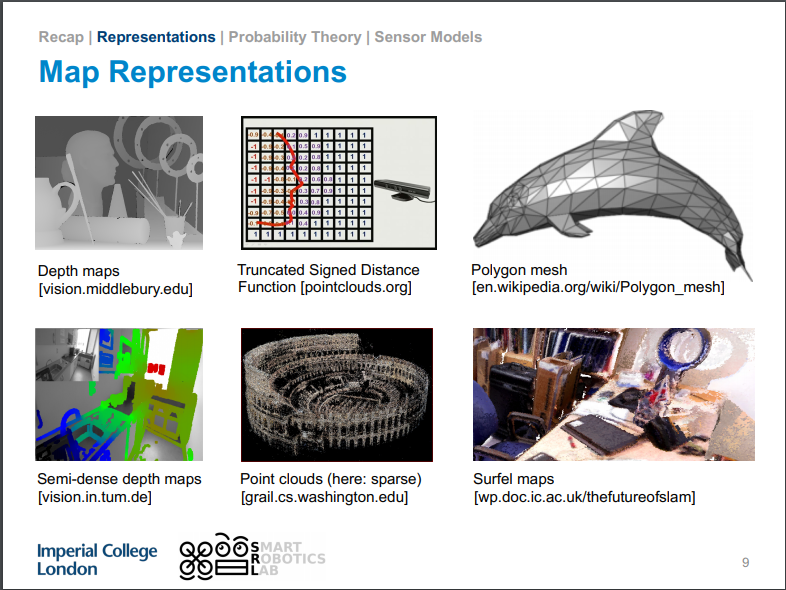
\includegraphics[scale=0.3]{Images/Literature/AdvancedRobotics_Maps.png}
%	\end{center}
%	
%\end{figure}

\subsection{Existing Work}
A review of SLAM techniques can be found in \cite{Cadena2016}, which also outlines the standard formulation of the SLAM problem as that of a Maximum a posteriori (MAP) estimation. The formulation relies on Bayes theorem, and using the prior knowledge of the robots pose to maximize the likelihood to estimate the current position of the robot. The variables required to estimate the position are the robot poses, the position of landmarks and the calibration parameters of the sensors.

In order to build an accurate map of the surroundings, the calibration of the sensors providing the measurements is a crucial step. The choice of sensors also matter, as the type of data returned by the sensor may affect the computational complexity of the SLAM algorithm. As such, it is common to have a module in the system that deals with the extraction of relevant features from the sensor data.

A fairly common assumption in SLAM approaches is that the world is static and remains unchanged as the robot moves. This becomes an issue with the goal of this project, which hopes to achieve the ability to detect human objects walking around the wheelchair. This issue will be addressed in a later section.

\subsection{Visual SLAM}
Visual SLAM (vSLAM) is an implementation of SLAM that relies on visual inputs only. As stated in \cite{Taketomi2017}, vSLAM is suitable for AR due to the low computational algorithms that can be implemented on the limited resources of an AR headset. The technique of vSlam is mainly composed of three modules:

\paragraph{Initialization}
In the initialization stage, camera pose estimation is conducted, to transform objects in a 2D image from the camera into a 3D co-ordinate system that the robot understands. This process determines the position and orientation of the camera relative to the object. A part of the environment is reconstructed as part of the initial map using the global co-ordinate system of the robot.

\paragraph{Tracking}
Here, the reconstructed map is used to estimate the pose of the camera with respect to the map. Feature mapping or feature tracking is conducted on the images in order to get a 2D-3D correspondence between the image and the map. The camera pose can then be calculated from the correspondences by solving the Perspective-n-Point problem \citep{Nister2004}. This allows the system to identify where on the map the robot currently is.

\paragraph{Mapping}
When the robot passes through an environment that has previously not been mapped, the 3D structure of the surroundings is calculated from the camera images. The structures are then added to the existing map of the environment.



\section{Eyetracker Control}

\section{Augmented Reality Visualization}

\section{Competing Products}

\section{Hardware Specifications}



\newpage

\bibliographystyle{agsm}
\bibliography{FinalYearProject}


\end{document}